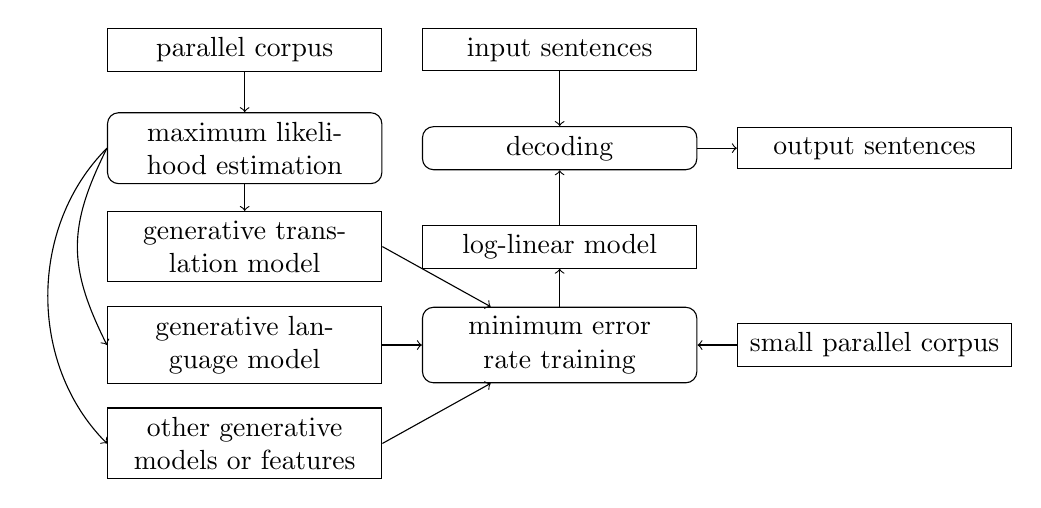
\begin{tikzpicture}[node distance=1.25cm]
	\tikzstyle{flow} = [text centered,text width=3.25cm]
	\tikzstyle{data} = [draw,rectangle,flow]
	\tikzstyle{process} = [draw,rectangle,rounded corners,flow]
	\node (corpus) [data] {parallel corpus};
	\node (mle) [process,below of=corpus] {maximum likelihood estimation};
	\node (tm) [data,below of=mle] {generative translation model};
	\node (lm) [data,below of=tm] {generative language model};
	\node (features) [data,below of=lm] {other generative models or features};
	\node (mert) [process,right of=lm,node distance=4cm] {minimum error rate training};
	\node (discriminative) [data,above of=mert] {log-linear model};
	\node (decoding) [process,above of=discriminative] {decoding};
	\node (input) [data,above of=decoding] {input sentences};
	\node (output) [data,right of=decoding,node distance=4cm] {output sentences};
	\node (dev) [data,right of=mert,node distance=4cm] {small parallel corpus};
	
	\draw[->] (corpus) -- (mle);
	\draw[->] (mle) -- (tm);
	\draw[->] (mle.west) .. controls +(-0.5,-1) and +(-0.5,1) .. (lm.west);
	\draw[->] (mle.west) .. controls +(-1,-1) and +(-1,1) .. (features.west);
	\draw[->] (tm.east) -- (mert);
	\draw[->] (lm.east) -- (mert.west);
	\draw[->] (features.east) -- (mert);
	\draw[->] (mert) -- (discriminative);
	\draw[->] (discriminative) -- (decoding);
	\draw[->] (input) -- (decoding);
	\draw[->] (dev) -- (mert);
	\draw[->] (decoding) -- (output);
\end{tikzpicture}